% !TeX spellcheck = fr_FR
\chapter{L'épée chinoise}\label{ch:epeechinoise}

On peut définir de manière générale une épée comme étant une arme blanche utilisée de taille ou d'estoc, avec une lame au moins aussi longue que le bras et une poignée courte.

On trouve des traces archéologiques de l'utilisation d'épées dès l'Âge du Bronze, tant dans le monde occidental qu'en Chine.

Depuis cette période reculée jusqu'au début du XX\textsuperscript{e} siècle, lorsqu'elles cessèrent d'être utilisées au combat, les épées ont évolué en parallèle des techniques martiales. 
L'escrime d'une période historique particulière était adaptée au type d'épée disponible à cette époque tout en étant profondément enracinée dans son contexte social et culturel.

Le \Taijijian{} a donc naturellement adopté le type d'épée à deux tranchants, ou \Jian{}, en usage à l'époque en Chine.
Bien qu'il n'y ait jamais eu dans l'histoire d'épées conçues spécifiquement pour le \Taijijian{}, ces épées chinoises à double tranchant sont pourtant de nos jours souvent appelées abusivement épées de \Taiji{}.

\section{Du champ de bataille au jardin public}
Je n'entrerai pas dans des considérations historiques approfondies sur l'escrime chinoise.
D'autres auteurs plus érudits que moi ont déjà publié sur le sujet des travaux plus précis et complets que tout ce que je pourrais écrire ici. Le lecteur intéressé trouvera de plus amples détails dans l'ouvrage de Peter Lorge \textit{Chinese Martial Arts: from Antiquity to the Twenty-First Century} et celui de Scott Rodell, \textit{Chinese Swordsmanship}. 

Après avoir dominé les champs de bataille chinois jusqu'à la fin du XIX\textsuperscript{e} siècle et au début du XX\textsuperscript{e}, les armes blanches furent supplantées par les armes à feu modernes et l'artillerie. L'application pratique de l'escrime chinoise déclina rapidement dès le début du XX\textsuperscript{e} siècle. 
\ChenWeiming{}, dans son livre \textit{\'{E}pée du \Taiji{}}, publié pour la première fois en 1928, ne mentionne l'escrime que pour préciser que \YangChengfu{} ne l'a jamais enseignée, et que lui même écrirait un autre livre sur le sujet lorsqu'il aurait acquis suffisamment d'expertise dans cette discipline. Autant que je sache, ce livre n'a jamais été écrit.
Dans les années 1930 et 1940, les manuels chinois d'épée déplorent que cet art antique soit presque totalement perdu.

\`{A} la même époque, alors que la Chine subissait l'influence des empires occidentaux, qu'elle était envahie par les troupes japonaises, puis ravagée par la guerre civile, les arts martiaux chinois devenaient un symbole de fierté nationale, tandis qu'ils se transformaient progressivement en disciplines pour l'éducation physique, la santé et le développement personnel.

La boxe et la lutte prirent bientôt le pas sur l'entraînement aux armes qui se réduisit à une simple pratique d'enchaînements en complément des arts martiaux à mains nues.
Les instructeurs en arts martiaux ne formaient plus guère de combattants, ils s'attachaient maintenant avant tout à renforcer leur nation en tonifiant leurs compatriotes par de saines pratiques tout en affirmant la supériorité de la tradition chinoise.
L'utilisation appliquée de l'escrime n'était plus un objectif, et les mouvements agiles, athlétiques et démonstratifs s'en trouvèrent favorisés au détriment d'une recherche de l'efficacité en combat.
Des épées légères, à la lame extrêmement flexible, furent utilisées de plus en plus fréquemment, jusqu'à devenir la norme.

Bien qu'il n'y ait à ma connaissance aucune trace écrite d'un art martial appelé \Taijiquan{} avant le XIX\textsuperscript{e} siècle, les principes du \Taiji{} circulaient certainement déjà depuis fort longtemps lorsqu'ils furent rassemblés en un système martial cohérent par la famille \Chen{} de \Chenjiagou{} et, plus tard, formalisés dans les textes connus de nos jours sous le nom de Classiques du \Taiji{}.

Dès le XVI\textsuperscript{e} siècle, le général \QiJiguang{} (1527\textendash{}1587), dans son \textit{Nouveau Manuel d'Efficacité Militaire}, énumère des techniques dont le nom sonne familièrement aux oreilles de tout pratiquant de \Taijiquan{}. Il n'est pas certain toutefois que \QiJiguang{} parlait effectivement de \Taijiquan{} ou de son ancêtre, ni s'il  s'agit d'une simple coïncidence ou d'une réutilisation ultérieure des mêmes noms de techniques.

Quoiqu'il en soit, on admet généralement que le \Taijiquan{} apparut et se développa entre la fin du XVII\textsuperscript{e} et le XIX\textsuperscript{e} siècle, pendant les dynasties \Ming{} et \Qing{}.

Le style \Yangjia{} \Michuan{}, fondement du présent travail, fut créé par \Yang{} \Luchan{}, probablement pendant la première moitié du XIX\textsuperscript{e} siècle.
Je n'ai aucune preuve manifeste que la forme d'épée \Kunlun{} du \Yangjia{} \Michuan{} date de cette époque, mais le poème qui en décrit les mouvements semble indiquer une origine relativement ancienne.
Le traité de \QiJiguang{} répertorie en effet de tels poèmes utilisés comme moyen mnémotechnique pour la pratique des formes.

\`{A} l'origine, les formes étaient utilisées pour entraîner les troupes de soldats à manœuvrer et combattre à l'unisson. Cependant, dès la dynastie des \Tang{}, les sessions d'entraînement devinrent une sorte de spectacle martial, non seulement comme démonstration de puissance militaire, mais aussi, comme un simple divertissement.
Les formes incorporèrent de plus en plus de techniques démonstratives, plus spectaculaires ou esthétiques qu'efficaces, pour le plus grand plaisir des spectateurs qui n'étaient souvent pas eux mêmes des pratiquants d'arts martiaux. 
Cet intérêt a persisté jusqu'à nos jours dans la littérature, l'opéra chinois, le cinéma, et, bien entendu, dans les inévitables démonstrations de toute rencontre d'arts martiaux qui se respecte.

De nos jours, comme tout autre art martial chinois, le \Taijijian{} a abandonné le champ de bataille pour le jardin public et, fort heureusement, l'entraînement à l'épée n'a plus pour objectif la préparation au combat.

Cependant, malgré leur indéniable dimension esthétique, les formes traditionnelles de \Taijijian{} furent conçues à l'origine pour développer des capacités martiales basées sur les principes du \Taiji{}, utilisant avec efficacité des épées dont les caractéristiques assuraient un compromis entre des coupes puissantes, des estocs précis et des mouvements rapides.

\section{Anatomie de l'épée \Jian{}}
La figure \ref{fig:sword_parts} montre les parties démontées d'une épée chinoise \Jian{} typique des dynasties \Ming{} et \Qing{}.

\begin{figure}[ht]
\centering
	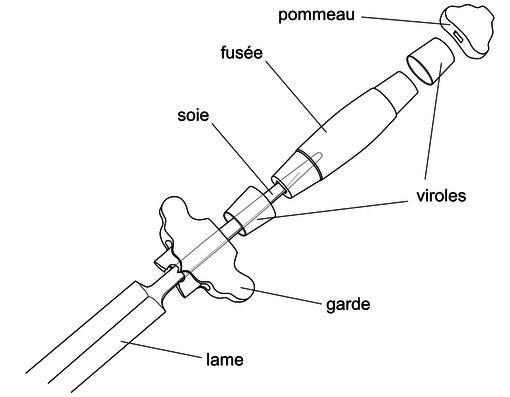
\includegraphics[width=0.69\textwidth]{../../Images/SwordParts/SwordPartsFr.pdf}
	\caption[Parties de l'épée]{Les parties de l'épée : La lame est prolongée par la soie sur laquelle sont emboités la garde, la poignée (fusée) et le pommeau. Les deux viroles sont deux anneaux de métal protégeant de l'éclatement les extrémités de la fusée. La garde protège la main portant l'épée. Généralement faite de bronze ou d'un métal similaire, elle est creuse et s'ouvre vers l'avant. La poignée, ou fusée, généralement faite de bois, a une forme de fuseau et est parfois recouverte d'un filigrane, de cuir, ou de peau de raie.
	Le pommeau, fabriqué dans le même métal que la garde joue un rôle primordial dans l'équilibre et le comportement de l'épée en contrebalançant le poids de la lame.}
	\label{fig:sword_parts}
\end{figure}

La principale particularité de la lame de l'épée chinoise tient dans ses deux tranchants quasiment parallèles. De 3 à 4 cm à la base, la largeur de la lame ne décroit que jusqu'à 2 à 3 cm près de la pointe, où les tranchants s'incurvent rapidement en une pointe acérée. 
Pour une lame de 70 à 80 cm, l'angle entre les deux tranchants est à peine discernable, à l'opposé de la forme franchement triangulaire de nombreuses épées médiévales européennes. 

Traditionnellement, la section de la lame pouvait être lenticulaire ou en losange avec une arête franche. 

Certaines lames pouvaient aussi comporter une gouttière, qui selon une légende tenace, aurait servi à permettre au sang de s'échapper de la plaie.
Une autre fantasmagorie au sujet de ces gouttières prétend qu'elles permettaient d'éviter à la lame d'être prise dans la blessure à cause d'un supposé phénomène de succion ou une hypothétique contraction des muscles blessés.
Je dois dire que j'ai de sérieux doutes sur la capacité d'un muscle entaillé à se contracter de manière significative autour d'une lame tranchante sans occasionner plus de dommages. Et en supposant qu'il le puisse, il n'y a aucune raison pour qu'une lame affûtée ne puisse pas s'ouvrir facilement un chemin vers la liberté.

La vérité est beaucoup moins fascinante : la gouttière permet d'alléger la lame sans compromettre sa solidité. \'{E}videmment, le moyen le plus facile pour réduire le poids de la lame est d'en diminuer l'épaisseur. Toutefois, la flexibilité de la lame en serait augmentée ce qui, au delà d'un certain degré, n'est pas souhaitable. Le profil des tranchants serait de même aplati, avec des conséquences possibles sur leur solidité. 
La gouttière autorise une lame plus légère avec un effet négligeable sur sa flexibilité et le profil des tranchants.
Par exemple, une gouttière de 1 cm de large et 2 mm de profondeur, sur deux tiers d'une lame lenticulaire de 75 cm représenterait un volume d'environ \unit{10}{\centi\meter\cubed}. La densité de l'acier étant de \unit{7,3}{\kilo\gram \per \deci\meter\cubed} à \unit{7,8}{\kilo\gram \per \deci\meter\cubed} selon sa composition et les traitements auxquels il a été soumis, une telle gouttière de chaque côté de la lame en aurait réduit le poids d'environ 150 g sans affecter le profil de ses tranchants. (voir figure \ref{fig:blade_section}) 
C'est loin d'être négligeable si on considère qu'une lame plus légère permet aussi d'alléger la garde et le pommeau. Ainsi, une telle gouttière permettrait au forgeron de monter une épée de 900 g, le poids habituel d'une épée chinoise historique, avec le même profil et la même longueur qu'une épée de plus de 1 kg sans la gouttière.

\begin{figure}[ht]
\centering
	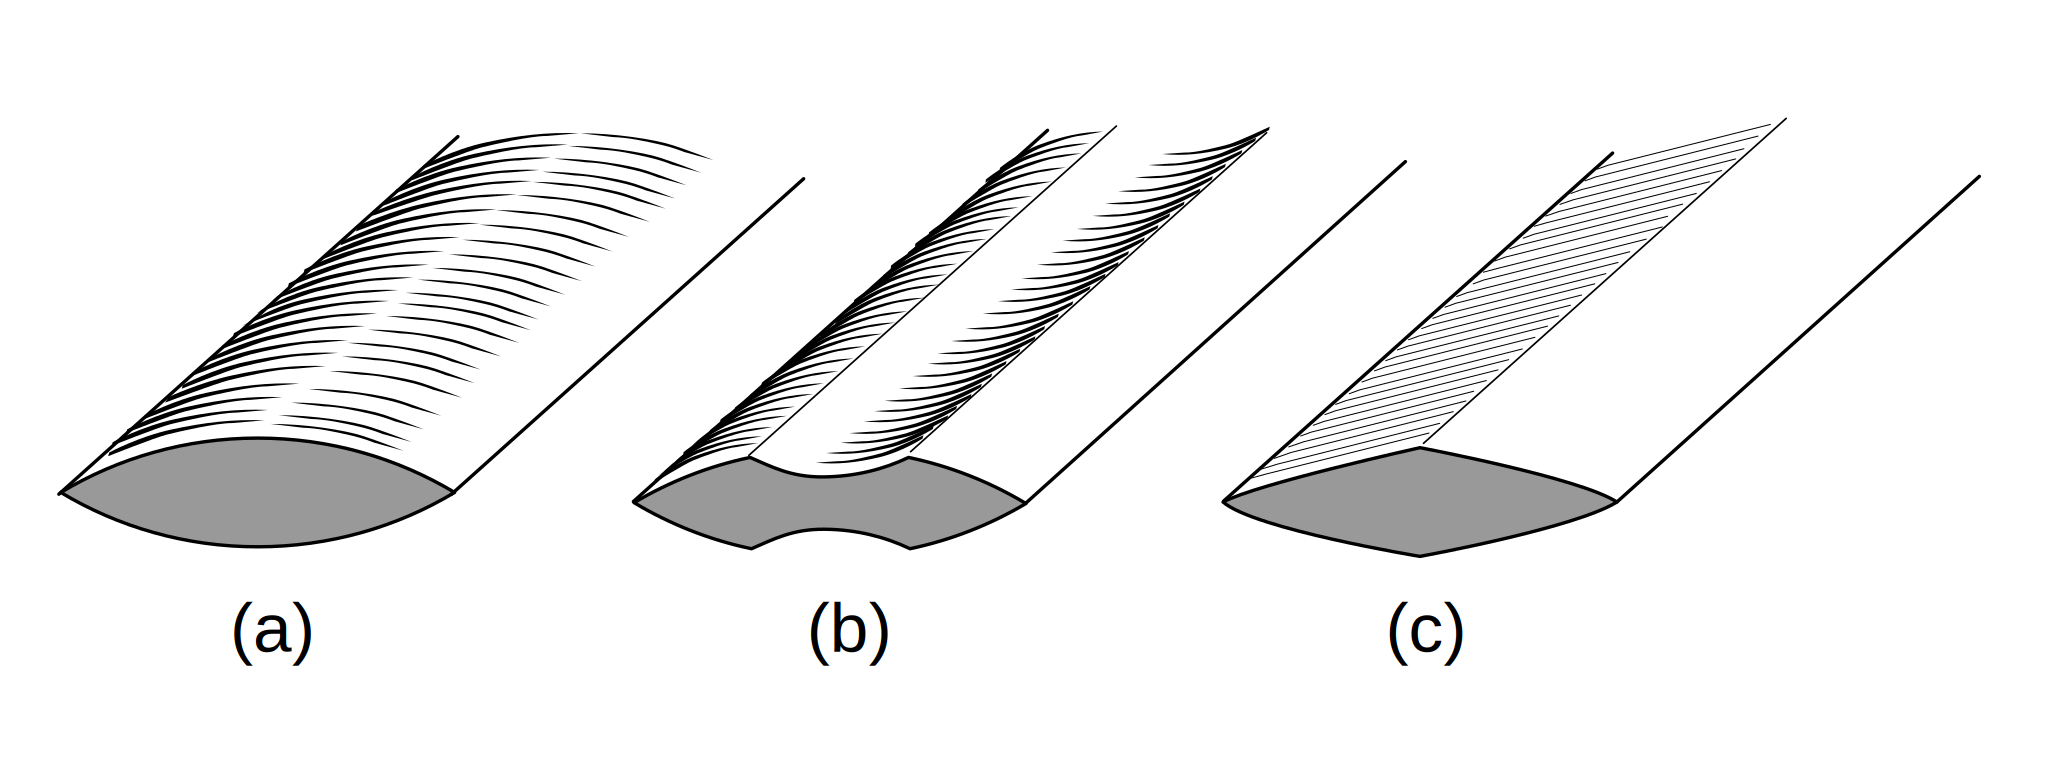
\includegraphics[width=0.69\textwidth]{../../Images/BladeSection/BladeSection.pdf}
	\caption[Sections de lame]{Sections de lames: (a) Lenticulaire. (b) Cette lame lenticulaire présentant une gouttière a le même profil de tranchants que la lame représentée en (a), mais elle est significativement plus légère grâce à la gouttière. (c) Losange.\\
	NB : pour des raisons de clarté, l'épaisseur des lames a été exagérée sur cette figure.}
	\label{fig:blade_section}
\end{figure}

Si le profil de la lame peut avoir une influence sur la durabilité des tranchants, le type d'acier dont la lame est faite affectera également leur solidité.
Avec un acier trop doux, les tranchants risquent de plier et de s'émousser après quelques coupes seulement. Pour durer les tranchants doivent être en acier durci, mais celui-ci étant cassant, il n'est pas envisageable de forger une lame exclusivement avec de l'acier dur. 
Un compromis est donc nécessaire entre la dureté de la lame, sa souplesse et son élasticité.

Notons bien qu'élasticité n'est pas synonyme de flexibilité : l'élasticité est la capacité de la lame à plier puis à revenir à sa forme d'origine. Si la limite d'élasticité est dépassée, la lame conserve une courbure ou se brise.
La lame doit être assez dure pour conserver des tranchants affûtés tout en étant suffisamment résiliente et élastique pour supporter des coups puissants et des chocs sans casser ni prendre une courbure définitive. 

En substance, l'acier est du fer additionné de 0,1\% à 2\% de carbone.  Il est aussi possible d'y allier d'autres métaux en faible quantité, comme le chrome, le nickel, le manganèse, etc.
La présence de ces éléments peut, malgré leur faible proportion, changer radicalement les propriétés mécaniques de l'acier conjointement avec les traitements par la chaleur.

Le \index{trempage}trempage est un processus consistant à chauffer la lame à haute température et à la refroidir rapidement par immersion dans de l'eau.
Suite à ce traitement, l'acier prend une structure cristalline particulière le rendant plus dur, mais aussi plus fragile.
D'autre part, comme il est impossible de refroidir instantanément et de manière homogène la totalité de la lame, le trempage crée aussi dans le métal des tensions persistantes qui risquent de fragiliser la lame.
Pour relâcher ces contraintes sans inverser les effets du trempage, il est possible d'appliquer à la lame un second traitement, appelé \index{recuit|see {revenu}}recuit ou \index{revenu}revenu. Il s'agit de chauffer à nouveau la lame à une température inférieure à celle du trempage avant de la laisser refroidir lentement, de manière à retrouver une bonne résilience. 

La technique appelée \index{trempage!trempage différentiel@\textit{trempage différentiel}}trempage différentiel constitue une alternative à ces deux traitements successifs. Renommée pour son utilisation dans la fabrication des sabres japonais, cette technique était à l'origine également utilisée en Chine.
Lors du trempage différentiel, seuls les tranchants sont soumis au choc thermique grâce à l'application d'argile sur la partie centrale de la lame, qui, ainsi protégée, conserve sa souplesse et son élasticité tandis que les tranchants sont durcis par le trempage.

Au Moyen-Âge en Europe, des tranchants d'acier durci étaient parfois soudés sur une âme en acier doux ou en fer. Autant que je sache, cette technique n'a été utilisée en Chine que pour les sabres.
La fabrication des épées droites chinoises faisait traditionnellement appel au procédé appelé \SanMei{}. La lame était constituée de trois couches d'acier soudées entre elles : une mince couche centrale dure formant les tranchants, entourée de deux couches d'acier doux ou de fer qui empêchaient qu'elle ne se brise sous des coups violents en donnant à la lame une structure élastique.

\section{Équilibre et propriétés dynamiques}
L'équilibre d'une épée est traditionnellement exprimée par la position de son 
centre de gravité (CG), aussi appelé centre d'inertie. Pour une épée de type \Jian{}, il se situe généralement entre 10 et 20 cm en avant de la garde, mesuré à partir de l'extrémité avant de la poignée.

Mais je pense qu'on donne habituellement trop d'importance à la position du CG. Bien que le CG joue un rôle important dans la manipulation de l'épée, il est loin d'être l'élément principal ayant une influence sur sa maniabilité. Alors que le CG d'un objet décrit son équilibre statique et comment il répond à l'application globale d'une force indépendamment de sa forme, les propriétés dynamiques de rotation dépendent aussi de la distribution des masses et de la forme. C'est la raison pour laquelle une barre et une boule homogènes ne se comportent pas de la même manière bien qu'elles aient toutes deux un CG confondu avec leur centre géométrique.

Les propriétés dynamiques d'une épée sont donc bien plus essentielles et déterminent la façon dont elle peut être maniée, comment elle bouge, comment elle tourne et répond aux actions exercées sur la fusée. En fait, il n'est pas rare de trouver des épées ayant un CG à la même distance de la poignée mais produisant des sensations radicalement différentes quand on les manipule.

Mais la mesure de la grandeur physique correspondant à ces propriétés dynamiques, le moment d'inertie, n'est pas particulièrement aisé, et une fois mesurée, l'interprétation de cette valeur scientifique en termes pratiques de manipulation d'une épée est loin d'être évidente.

Une façon précise de mesurer le moment d'inertie d'une épée est le test du pendule, qui consiste à en mesurer la période d'oscillation naturelle autour d'un axe situé à une distance donnée du CG. Après quelques calculs mathématiques, on obtient une valeur qui, pour être honnête, n'est guère parlante sans point de référence. De plus amples recherches seront assurément bienvenues sur le sujet.

Une manière plus simple d'observer les propriétés dynamique d'une épée est le test des points pivots. Bien qu'il soit bien moins précis, il a l'avantage de donner quelques indications sur la façon dont ces propriétés ont une influence sur la manière dont l'épée réagira aux actions exercées sur la poignée.

Pour réaliser ce test, tenez légèrement l'épée entre le pouce et l'index, et imprimez-lui avec légèreté une oscillation latérale. Vous pourrez remarquer dans la lame un point qui ne bouge pas : il s'agit du point pivot relatif à l'endroit où vous tenez la fusée (voir figure \ref{fig:pivot_points}).

Un changement de position des doigts sur la poignée déplacera le point pivot. En manipulant une épée, il est donc possible de contrôler la position du centre de rotation de l'épée en ajustant la position et la direction de l'action exercée par votre prise sur la poignée.

Les points pivots relatifs à la poignée se trouvent en général localisés dans la première moitié de la longueur de l'épée en partant de la pointe.

\begin{figure}[ht]
\centering
	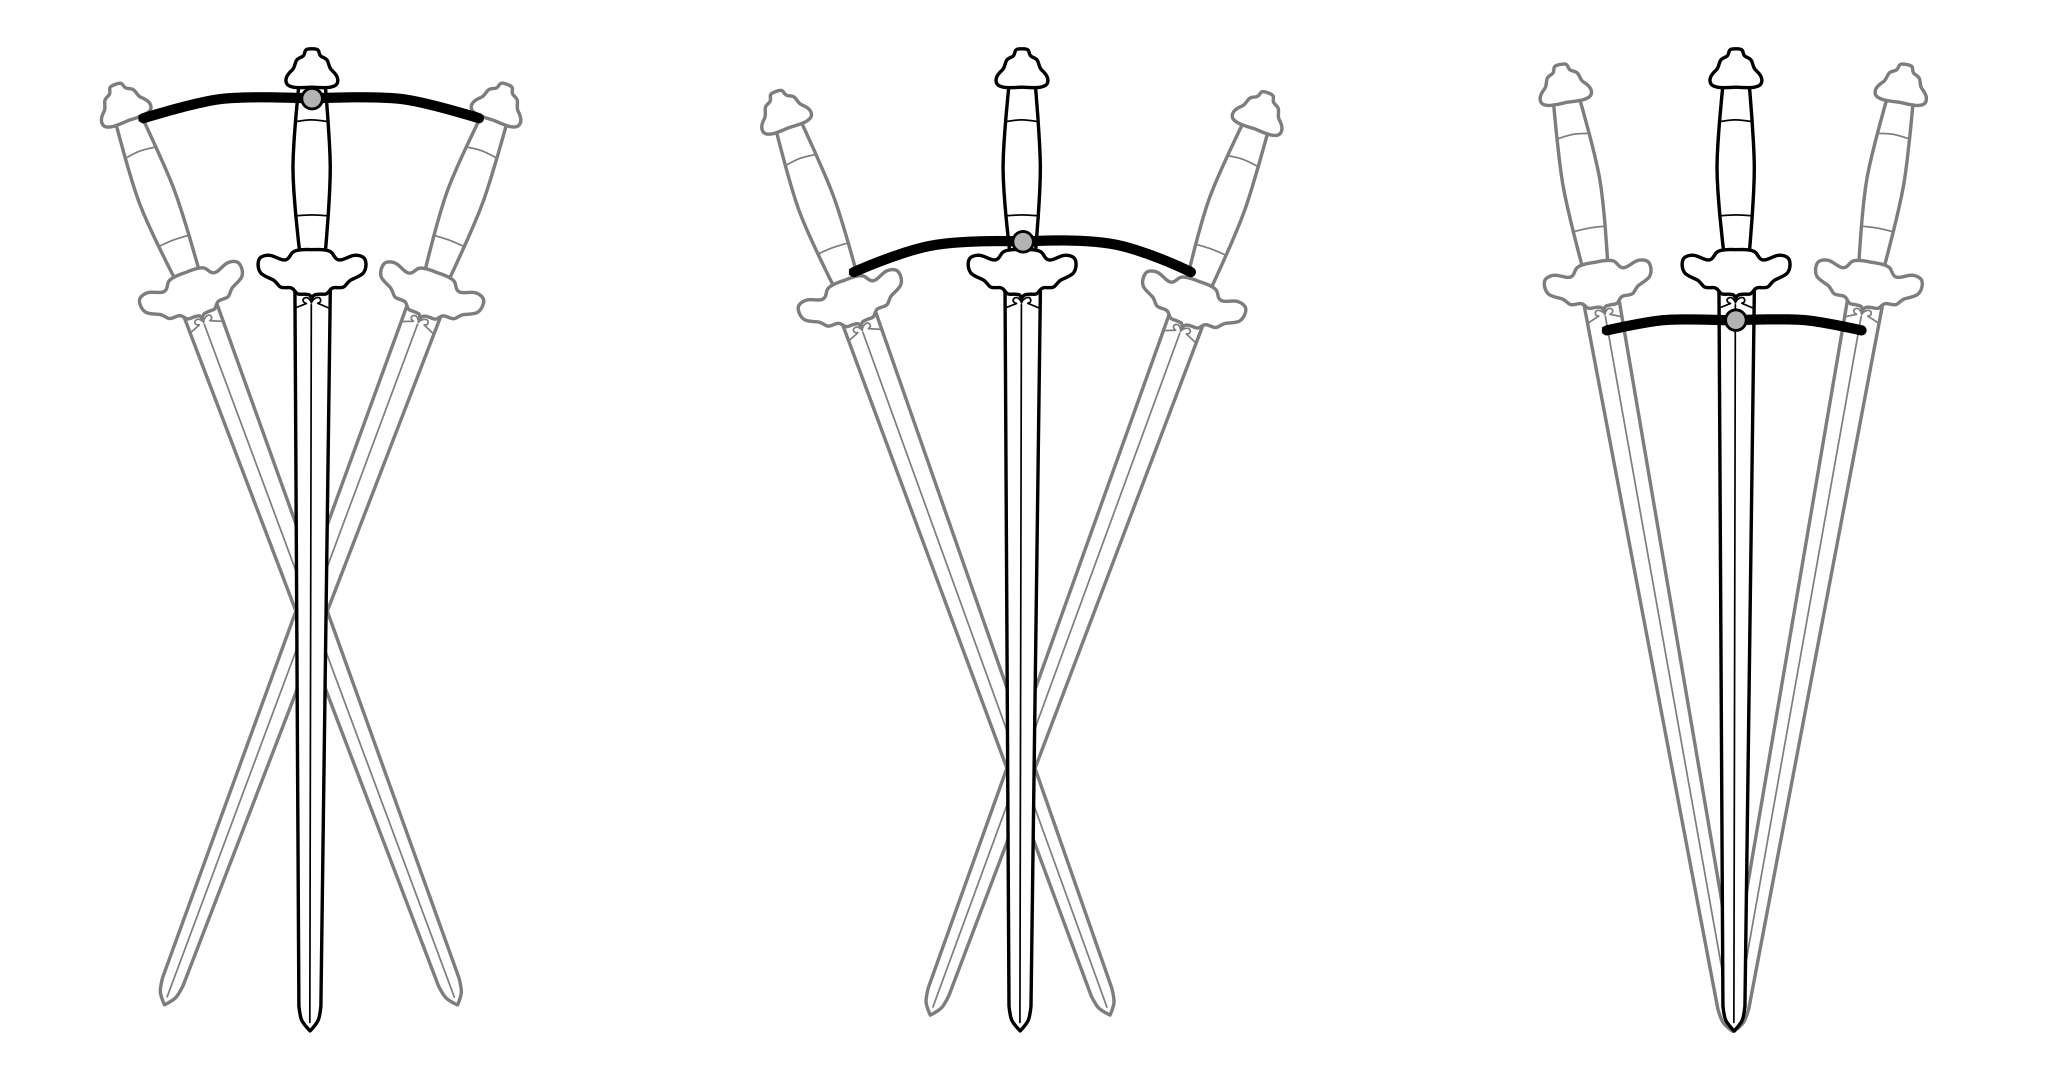
\includegraphics[width=0.80\textwidth]{../../Images/PivotPoints/PivotPoints.pdf}
	\caption[Points pivots]{Un point pivot est le centre de rotation naturel de l'épée selon l'emplacement et la direction d'une action exercée sur la fusée. Si l'épée est tenue près du pommeau et agitée latéralement, le point pivot est proche du centre de la lame (gauche). Tenir l'épée près de la garde déplace le point pivot plus loin vers la pointe (milieu). Pour placer le point pivot dans la pointe, une action latérale doit être exercée environ 2 cm en avant de la garde (droite). Bien que cela puisse sembler désavantageux, un ajustement approprié de la prise et une action oblique sur la fusée permet tout de même de contrôler ce point. De plus, il est ainsi possible de conserver sa pointe en ligne en tirant un estoc tout en contrôlant la lame de l'adversaire avec la garde.}
	\label{fig:pivot_points}
\end{figure}

Leur position est déterminée par la distribution des masses le long de l'épée et en particulier par les masses relatives de part et d'autre de la prise. Les facteurs affectant cette distribution sur une lame non fourbie sont la forme et les dimensions de sa section, comment elle diminue en largeur et épaisseur depuis la soie jusqu'à la pointe, ainsi que la taille relative de la soie. L'ajout d'un pommeau sur une lame non montée, même s'il est relativement léger, va modifier de façon importante la dynamique de l'épée. Non seulement le CG va se rapprocher de la garde, mais les points pivots vont être déplacés vers la pointe. Toutefois, un pommeau trop lourd risque de les déplacer trop en avant, voire même au delà de la pointe. \`{A} l'opposé, un pommeau trop léger rendrait difficile ou même impossible l'obtention d'un point pivot contrôlant exactement la pointe. 
Une amplitude correcte des points pivots permettant un bon contrôle de la lame nécessite donc un ajustement précis de la forme de la lame et des poids respectifs de celle-ci et du pommeau.

Le lecteur intéressé trouvera de plus amples informations sur ce sujet dans le livre \textit{Das Schwert \textendash{} Gestalt und Gedanke/The Sword \textendash{} Form and Thought} publié par le \textit{Deutches Klingen Museum} à Solingen. Bien qu'il ne présente exclusivement que des épées occidentales de différentes périodes, cet ouvrage présente une mine d'informations concernant l'équilibre et la dynamique d'une épée tout à fait applicable aux épées chinoises.

\section{Choisir une épée de \Taijijian{}}
%\subsection{Which sword for which practice?}
On trouve sur le marché une grande variété d'épées pour la pratique du \Taijijian{}. En choisir une est habituellement une affaire de goût et de budget.
Ces épées sont toutefois pour la plupart fort différentes des armes qui étaient encore en usage lorsque les formes traditionnelles de \Taijijian{} furent créées.
Beaucoup sont très approximativement équilibrées et sont soit trop légères ou trop lourdes.
Si le poids d'une épée d'entraînement n'est après tout pas si important et devrait être adapté de toute manière à l'expérience et aux capacités physiques du pratiquant, l'équilibre et les qualités dynamiques de l'épée ne devraient jamais être ignorées.
Assurer la sécurité des pratiquants d'exercices avec partenaire ou d'assauts libres constitue également une priorité absolue.

Il est probable que les pratiquants s'intéressant vraiment à tous les aspects du \Taijijian{} possèderont au final au moins deux épées, une pour la pratique de la forme, et l'autre pour les exercices avec partenaire et les assauts libres.

\subsection{Pratique de la forme}\index{forme!choisir une épée@\textit{choisir une épée}}
Comme les mouvements des enchaînements traditionnels étaient adaptés à l'équilibre des épées de l'époque de leur création, la pratique de la forme avec une telle arme, même passablement lourde, ne devait pas exiger d'effort particulier lorsque les principes du \Taiji{} étaient respectés.

Pratiquer de nos jours avec une épée de dimensions, poids et équilibre similaires à ceux d'armes historiques ne peut donc que nous rapprocher de l'esprit originel des formes traditionnelles.
Il est certes bien plus exigeant de manipuler une telle épée qu'une lame très légère, cela n'en est pas moins une occasion incomparable et stimulante d'approfondir notre compréhension de cet art et d'incarner les principes du \Taiji{}.

Cependant, bien qu'une épée lourde puisse être un meilleur guide qu'une épée légère pour la pratique de la forme, elle laisse aussi moins passer les erreurs techniques et l'excès de tension musculaire.
Le poids de l'épée devrait donc être adapté à l'expérience du pratiquant et à sa forme physique. Il n'est pas judicieux pour un débutant de pratiquer avec une épée tellement lourde qu'elle ne pourrait que sanctionner ses articulations et ses muscles au moindre mouvement incorrect qu'il ferait.
Ainsi, une épée de bois ou d'acier bon marché conviendra parfaitement pour débuter et mémoriser la forme, mais deviendra vite limitante pour un approfondissement de la pratique.
Lorsqu'il aura acquis une expérience suffisante, le pratiquant aura tout avantage à passer à une épée correctement équilibrée et d'un poids approximatif de 700 à 900 g, équivalent à celui d'armes historiques.

De même, les débutants apprenant la forme et les bases risquent d'être gênés inutilement par une longue lame et devraient favoriser des épées plus courtes. Les pratiquants avancés, si leur prise est vraiment relâchée, devraient toutefois être capables de s'accommoder aisément d'une lame plus longue, à condition que sa longueur ne soit pas excessive.

Une règle classique consiste à déterminer la bonne longueur de lame en tenant l'épée verticalement le long du bras gauche, comme pour l'ouverture de la forme. La pointe de la lame devrait alors se trouver en face de l'oreille. En résumé, ceci est tout à fait équivalent au fait de s'assurer que la lame est en moyenne plus longue que la longueur du bras de la plupart des adversaires potentiels. Ceux-ci ne pourraient ainsi pas se protéger d'un estoc en le bloquant au niveau de la garde.
Quoiqu'il en soit, une lame de 70 à 75 cm devrait convenir à la plupart des pratiquants.

La présence d'un \index{pompon}pompon dépendra du style pratiqué. Certains styles en utilisent un, d'autres pas, à l'instar du \Yangjia{} \Michuan{}. 

On a dit beaucoup de choses sur le rôle du pompon. Il est largement admis que, pendant la pratique de la forme, la manière dont le pompon bouge donne des indications sur la qualité de mouvement du pratiquant.
Je suis prêt à accepter cet argument qui fait du pompon un outil pédagogique pour équilibrer l'intention entre la pointe de l'épée et la poignée. Mais si le pompon accapare trop l'attention du pratiquant, celui-ci risque fort de finir par pratiquer une forme de pompon. 

Je suis bien moins convaincu par d'autres explications telles que l'utilisation du pompon pour détourner l'attention de l'adversaire. Je préfère personnellement menacer l'adversaire avec la lame, qui est bien plus impressionnante et qui, contrairement au pompon, est tranchante et ne peut pas être saisie.

En réalité, si on se réfère aux représentations historiques d'épées et de bretteurs, il semble que le pompon soit d'une invention assez récente. Je penche pour une évolution décorative des dragonnes qu'on peut voir sur des images plus anciennes et qui servaient à assurer l'épée dans la main pendant le combat.
En tout état de cause, n'utilisant pas de pompon, je ne peux que suggérer de faire à ce sujet ce que recommande votre style.

\subsection{Exercices avec partenaire et applications martiales}\index{exercices avec partenaire!choisir une épée@\textit{choisir une épée}}\index{applications martiales!choisir une épée@\textit{choisir une épée}}
Il est possible de pratiquer avec la même épée que la forme, des exercices simples avec partenaire tels que les épées collantes, guider et suivre, etc. tant qu'il n'y a aucune attaque lancée au visage ou vers la partie supérieure du corps.

Je recommande toutefois vivement de réserver les exercices sans protections strictement à des pratiquants expérimentés et entraînés, ayant l'habitude de pratiquer ensemble. Dans tous les autres cas, l'utilisation d'une épée conçue pour le travail avec partenaire et des protections adéquates  \textendash{} au minimum un masque d'escrime et des gants \textendash{} est absolument nécessaire pour réduire les risques d'accident.

Des épées rigides non tranchantes dont la pointe a été recouverte d'une pièce de cuir peuvent constituer un bon compromis pour un budget limité. Toutefois, il faut garder à l'esprit que ces épées n'ont pas été conçues pour cet usage et qu'elles peuvent s'avérer dangereuses sans les protections et précautions adéquates. Un accident est toujours possible, et quiconque utilise de telles épées pour un travail avec partenaire le fait à ses propres risques. Notez bien qu'il n'est pas recommandé d'utiliser ici ce qu'on appelle une lame flexible. Non seulement ces lames ne sont pas adaptées au travail avec partenaire, elles sont aussi tellement fines qu'elles en sont presque tranchantes.

Contrairement à ce qu'on pense généralement, les épées de bois ne sont pas réellement plus sûres puisqu'en raison de leur rigidité, elles ne peuvent absorber efficacement le choc d'un estoc. De plus, l'épaisseur de lame des épées de bois interdit une bonne sensation du contact.

La meilleure option reste assurément l'utilisation d'épées conçues spécialement pour le travail avec partenaire. Leurs tranchants épais et arrondis ainsi que leur pointe retournée les rendent relativement sécurisées à condition de porter au minimum un masques d'escrime et des gant rembourrés. Une veste d'escrime rembourrée apportera une protection supplémentaire permettant des exercices plus intenses et dynamiques. 
D'autre part, avec un poids supérieur à 800 g, elles autorisent moins que des épées légères les entorses à une réalisation correcte des techniques dans le respect des principes, ce qui doit être vu comme un avantage dans la perspective des applications et exercices techniques.



\subsection{Assaut libre}\index{assaut libre!choisir une épée@\textit{choisir une épée}}
Bien qu'on puisse pratiquer des jeux doux et tranquilles avec des lames non protégées ou des épées mouchetées à l'aide d'une pièce de cuir, je recommande vivement de toujours utiliser des épées spécialement conçues pour l'assaut libre (\textit{sparring}) et des protections appropriées pour la pratique de l'escrime (masque d'escrime, gant rembourrés, veste d'escrime rembourrée).
Sans protections efficaces ni précautions, même en restreignant volontairement les attaques aux parties basses du corps, des réactions instinctives peuvent être la cause d'accidents aux conséquences graves. 

Les épées de bois ne sont pas plus adaptées aux assauts libres qu'aux exercices avec partenaire. Des coupes vigoureuses et non contrôlées heurtant les doigts ou un os ne sont pas moins douloureuses ou dangereuses qu'avec une épée en acier. Sur un estoc, au contraire d’une lame d’acier, une épée de bois ne plie pas et toute l’énergie du choc est transmise à la cible au lieu d’être partiellement dissipée par la lame.

Une bonne épée pour l'assaut libre doit avoir une pointe arrondie ou retournée et des tranchants épais et arrondis pour permettre des estocs et coups de taille moins dangereux. Elle doit être suffisamment lourde pour obliger à utiliser des techniques correctes et empêcher des mouvements de poignet irréalistes similaires à ceux utilisés en escrime moderne au fleuret. Cependant, son équilibre doit permettre de réaliser toutes les techniques des formes traditionnelles de \Taijijian{} de manière naturelle avec des transformations vivaces et aisées.

Il existe maintenant des épées chinoises en acier conçues pour l'assaut libre et les exercices avec partenaire. Mon modèle favori, et celui que nous utilisons dans notre groupe, est produit par \textit{Péter Regenyei Armory}. Cette épée pour l'assaut (sparring \Jian{}) est le résultat d'une collaboration entre Mattias Nyrell, instructeur principal de \Jianfa{} du \textit{Historisk Fäktning i Linköping}, Péter Regenyei, forgeron renommé fabricant d'épées, et Peter Dekker, un antiquaire spécialisé dans les armes et armures de Chine et autres régions d'Asie, fondateur de \textit{Mandarin Mansion}.

La conception de cette épée s'inspire d'une \Tuanlianjian{} historique appartenant à la collection privée de Peter Dekker. Ces épées modestes et pratiques sont aussi connues sous le nom d'épées de milice puisqu'elle étaient probablement utilisées par des milices rurales pour défendre leurs biens et leurs villages. L'aspect des épée pour l'assaut de Péter Regenyei contraste donc fortement avec le style doré et parfois ampoulé de la plupart des épées chinoises sur le marché. Cependant, par leur simplicité, ces épées reflètent la beauté et la qualité de leur fabrication artisanale.

La lame de 73 cm de long aux bords presque parallèles possède une pointe retournée, une section en diamant aplati et des tranchants arrondis et épais de 1 à 2 mm. Ces bords épais et la pointe retournée assurent une bonne répartition de l'énergie dans les coupes et les estocs sur les protections. Cela ne constitue toutefois pas un sauf-conduit pour des coupes ou des estocs appuyés de toute force. En effet, bien que cette lame ait un certain degré de flexibilité, elle n'en est pas moins assez rigide et il peut être judicieux de porter un plastron, surtout pour les femmes, et un gorgerin en plus de la veste rembourrée habituelle.  

Malgré un poids de 800 à 900 g, cette épée semble plutôt légère dans la main, avec une forte sensation d'homogénéité du pommeau à la pointe. Le seul point qui pourrait demander un peu d'habitude est la section anguleuse de la poignée. Mais ceci peut en fait s'avérer un avantage en assaut libre pour mieux sentir l'alignement de la lame en portant des gants rembourrés.

Son excellent équilibre en fait une épée vivace et agile, très aisée à contrôler à condition d'être correctement connecté et de la mouvoir avec tout le corps et pas uniquement à partir du poignet ou du bras. Tous les mouvements et leurs transformations semblent naturels et dynamiques, que ce soit en déroulant la forme \Kunlun{} du \Yangjia{} \Michuan{} ou en assaut libre.

Je ne puis donc que recommander le pratiquant de \Taijijian{} passionné d'investir dans ce modèle d'épée. Pour tout dire, si vous ne deviez posséder qu'une seule épée, ce serait celle-ci: elle est en effet parfaite non seulement pour l'assaut et le travail avec partenaire, mais aussi pour la pratique de la forme.
